\chapter{商与对偶}

关于矩阵运算进阶的两讲我们将讲述线性代数这门课中关于矩阵计算问题的一些进阶内容. 需要注意的是,本节除了一些基本概念在之后讨论矩阵的秩时还有关键作用之外,大都是技巧性的内容,基本都已经脱离了之前描述的抽象空间和映射. 但我们仍需承认这些内容的重要性,因为运算技巧将会使得未来的很多性质的研究更为便捷. 同时我们也应当感到欣慰,我们终于从抽象空间一步一步如同搭积木一般走到了具象的运算,并且这是建立在了充分理解了矩阵背后的内在含义的基础上的.

本节我们首先介绍有关初等矩阵、分块矩阵和矩阵方程的相关内容. 本节是之后讨论矩阵的秩的重要基础,并且涉及一些很重要的算法和技巧,需要引起重视.

\section{线性空间的商}

\subsection{商空间的引入与仿射子集}

我们继续循着数学概念学习的自然路径,再来审视一个新的概念——商空间. 在第一讲中我们描述了一个非常重要的概念——等价类. 我们希望在一个线性空间$V$中构造等价类组成商集,并在商集中引入加法和数乘运算,使得商集构成线性空间,这便是本节要讨论的商空间的来由. 总结一下,我们这里有两个需求:其一是构造合适的等价关系,其二是构造合理的加法和数乘运算.

回忆集合的等价关系的建立,都是元素之间的关系. 例如等于关系是实数集合中的实数之间的关系,因此要在线性空间中建立等价关系,我们需要考虑两个元素(即向量)的关系. 我们可以考虑$V$的子空间$U$,并将关系$R$定义为
\[\forall\alpha,\beta\in V,\enspace\alpha\,R\,\beta\iff \alpha-\beta\in U.\]
即两个向量的差向量在一个规定的子空间中时称它们等价. 我们会很容易地验证出这个关系就是等价关系:
\begin{enumerate}
    \item (自反性) $\forall \alpha\in V,\enspace\alpha-\alpha=0\in U$,故$\alpha\,R\,\alpha$;

    \item (对称性) $\forall \alpha,\beta\in V,\enspace\alpha\,R\,\beta\implies \alpha-\beta\in U\implies \beta-\alpha=-(\alpha-\beta)\in U\implies \beta\,R\,\alpha$;

    \item (传递性) $\forall \alpha,\beta,\gamma\in V,\enspace\alpha\,R\,\beta,\enspace\beta\,R\,\gamma\implies \alpha-\beta\in U,\enspace\beta-\gamma\in U\implies \alpha-\gamma=(\alpha-\beta)+(\beta-\gamma)\in U\implies \alpha\,R\,\gamma$.
\end{enumerate}
证明只用到了线性空间的加法单位元、逆元性质且运算封闭. 接下来我们可以基于此定义这一等价关系的等价类:
\[\overline{\alpha}=\{\beta\in V \mid \beta\,R\,\alpha\}=\{\beta\in V \mid \beta-\alpha\in U\}=\{\beta\in V \mid \beta=\alpha+\gamma,\enspace\gamma\in U\}\]
最后一个集合还可以进一步写成$\{\alpha+\gamma \mid \gamma\in U\}$,我们记为$\alpha+U$,称之为$V$的仿射子集. 我们给出如下完整的定义:
\begin{definition}[仿射子集] \index{fangsheziji@仿射子集 (affine subset)}
    设$v\in V$,$U$是$V$的子空间,则$V$的\term{仿射子集}是$V$的形如$v+U$的子集,其中$v+U$定义为
    \[v+U=\{v+u \mid u\in U\}.\]
\end{definition}
根据我们之前的讨论,仿射子集就是我们在线性空间上定义的等价关系的等价类. 基于等价类的性质,我们有如下定理:
\begin{theorem}
    设$U$是$V$的子空间,$v,w\in V$,则以下陈述等价:
    \begin{enumerate}
        \item $v-w\in U$;

        \item $v+U=w+U$;

        \item $(v+U)\cap(w+U)\neq \varnothing$.
    \end{enumerate}
\end{theorem}

还需要强调的一点是,$(v+U)+(w+U)$与$(v+w)+U$是完全相同的集合,等价性是显然的,我们只需要展开写出仿射子集定义然后证明两个集合互相包含即可. 当然更一般的情形为
\[(v_1+U_1)+(v_2+U_2)+\cdots+(v_n+U_n)=(v_1+v_2+\cdots+v_n)+U_1+U_2+\cdots+U_n.\]

按照我们之前所说的学习数学的基本思路,在学习一个新的概念后我们会尝试考察它是否具有某些特别的性质,从而可以更深入地理解这一概念. 类似于线性空间我们介绍过原点的直线、平面然后介绍一般线性空间的基本结构是基和维数,我们从直观入手,然后逐步考察仿射子集的基本结构.

相信读者对``仿射''一词并不完全陌生,仿射变换实际上就是形如\[\vec{y}=A\vec{x}+\vec{b}\]的映射,其中$\vec{y},\vec{x},\vec{b}$为向量,$A$是一个矩阵. 实际上一元向量的情况就对应着一条斜率为$A$截距为$b$的直线.

事实上,若$V$为二维空间(平面),$U$为$V$的一维子空间,则其几何意义就是一条过原点的直线,而集合$v+U$实际上将原集合所有点沿着$v$的方向平移,可以得到截距不为0的直线,这就体现了``仿射''一词的意义. 高维空间则是同理,只是我们很难直观地看到这一点. 因此,我们也可以称仿射子集$v+U$\textbf{\heiti 平行于}$U$.

下面的例子给出了仿射子集的一种等价描述,基于此我们可以对仿射子集中向量的结构有更进一步的了解:
\begin{example}\label{ex:8:仿射子集性质}
    证明:$V$的非空子集$A$是$V$的仿射子集当且仅当对所有的$v,w\in A$和$\lambda\in\mathbf{F}$均有$\lambda v+(1-\lambda)w\in A$.
\end{example}

\begin{solution}

\end{solution}

事实上,结合我们之前所说的仿射子集几何意义,这一结论在平面上来看正是我们高中学习的平面向量中学习的三点共线的等价条件的同义表达:
\begin{theorem}
    设$P,A,B,C$是平面上四点,$P$与$A,B$不共线,则$C$与$A,B$共线等价于存在$\lambda\in\mathbf{R}$使得$\overrightarrow{PC}=\lambda\overrightarrow{PA}+(1-\lambda)\overrightarrow{PB}$.
\end{theorem}
同时我们发现仿射子集实际上是我们在数学分析或微积分学习的凸集的特殊形式,在凸集中我们只要求$\lambda\in[0,1]$,这里我们要求整个数域上的点都要有\autoref{ex:8:仿射子集性质} 所述的性质. 因此凸集的性质我们也可以用来研究仿射子集. 当然这不是线性代数中研究的内容,感兴趣的同学可以学习凸优化的相关课程进一步了解.

事实上在习题中我们将给出\autoref*{ex:8:仿射子集性质} 更一般的形式,我们可以回忆\autoref{thm:2:线性扩张构造子空间},就会发现仿射子集的结构和线性空间保留了一些相似性,即虽然不能像线性空间一样保证加法数乘运算封闭,但仿射子集一定是保证凸组合封闭的集合.

\subsection{商空间}

定义了等价类(即仿射子集)后,我们可以定义相应的商集(即由全体等价类构成的集合),我们称之为商空间:
\begin{definition}
    设$U$是$V$的子空间,则商空间$V/U$是指$V$的所有平行于$U$的仿射子集的集合,即
    \[V/U=\{v+U \mid v\in V\}.\]
\end{definition}
我们希望这些这一商集(商空间)真的构成线性空间,因此还需要定义加法和数乘运算. 定义是非常直接的:
\begin{definition}
    设$U$是$V$的子空间,则商空间$V/U$上的加法和数乘运算定义为:$\forall \alpha,\beta\in V$和$\lambda\in\mathbf{F}$,
    \begin{gather*}
        (\alpha+U)+(\beta+U)=(\alpha+\beta)+U, \\
        \lambda(\alpha+U)=(\lambda\alpha)+U.
    \end{gather*}
\end{definition}
我们很容易根据线性空间8条性质验证商空间在上述加法和数乘运算定义下构成线性空间,在此不再赘述. 特别注意这一线性空间的零向量是特别的,应当为$U$(即$\vec{0}+U$,一定注意不是$\vec{0}$,读者在验证商空间是线性空间时就会发现).

正常而言,在定义了一个线性空间后我们自然地想了解它的基本结构——基和维数,商空间也不例外. 我们通过下面这个定理来研究:
\begin{theorem}\label{thm:8:商空间维数}
    设$U$是有限维线性空间$V$的子空间,则
    \[\dim V/U=\dim V-\dim U.\]
\end{theorem}
这一定理的证明完全类似线性映射基本定理的证明,因此我之前一再强调这一思想的重要性. 我们的想法还是``设小扩大'':

\begin{proof}
    取$U$的一组基$\alpha_1,\alpha_2,\ldots,\alpha_s$,将其扩充为$V$的一组基$\alpha_1,\alpha_2,\ldots,\alpha_s,\alpha_{s+1},\ldots,\alpha_n$. 于是我们要证的转化为$\dim V/U=n-s$,即证明$V/U$的一组基的长度为$n-s$.

    类似于线性映射基本定理的证明,我们可以依靠直觉猜想. 我们猜想$V/U$的一组基为$\{\alpha_{s+1}+U,\alpha_{s+2}+U,\ldots,\alpha_n+U\}$. 这是很自然的想法. 我们只需要验证这组基的两个条件:线性无关和张成性:
    \begin{enumerate}
        \item 线性无关:设$\lambda_{s+1},\lambda_{s+2},\ldots,\lambda_n\in\mathbf{F}$,使得
              \[\lambda_{s+1}(\alpha_{s+1}+U)+\lambda_{s+2}(\alpha_{s+2}+U)+\cdots+\lambda_n(\alpha_n+U)=U.\]
              特别注意这里的零元是$\vec{0}+U=U$,实际上,上式等价于
              \[(\lambda_{s+1}\alpha_{s+1}+\lambda_{s+2}\alpha_{s+2}+\cdots+\lambda_n\alpha_n)+U=U.\]
              根据仿射子集定义,$\lambda_{s+1}\alpha_{s+1}+\lambda_{s+2}\alpha_{s+2}+\cdots+\lambda_n\alpha_n\in U$,因此可以被表示为$U$的基的线性组合,即
              \[\lambda_{s+1}\alpha_{s+1}+\lambda_{s+2}\alpha_{s+2}+\cdots+\lambda_n\alpha_n=\mu_1\alpha_1+\mu_2\alpha_2+\cdots+\mu_s\alpha_s.\]
              于是我们有
              \[\lambda_{s+1}\alpha_{s+1}+\lambda_{s+2}\alpha_{s+2}+\cdots+\lambda_n\alpha_n-\mu_1\alpha_1-\mu_2\alpha_2-\cdots-\mu_s\alpha_s=0.\]
              由于$\alpha_1,\alpha_2,\ldots,\alpha_n$是$V$的一组基,因此我们有$\lambda_{s+1}=\lambda_{s+2}=\cdots=\lambda_n=\mu_1=\mu_2=\cdots=\mu_s=0$. 从而$\alpha_{s+1}+U,\alpha_{s+2}+U,\ldots,\alpha_n+U$线性无关;

        \item 张成空间:$\forall\alpha+U\in V/U$,其中$\alpha\in V$,我们有$\alpha$可以被$V$的基线性表示为
              \[\alpha=\lambda_1\alpha_1+\lambda_2\alpha_2+\cdots+\lambda_n\alpha_n.\]
              于是
              \begin{align*}
                  \alpha+U & =(\lambda_1\alpha_1+\lambda_2\alpha_2+\cdots+\lambda_n\alpha_n)+U         \\
                           & =(\lambda_1\alpha_1+U)+(\lambda_2\alpha_2+U)+\cdots+(\lambda_n\alpha_n+U) \\
                           & =\lambda_1(\alpha_1+U)+\lambda_2(\alpha_2+U)+\cdots+\lambda_n(\alpha_n+U)
              \end{align*}
              因此$V/U$中任意元素均可被$\alpha_{s+1}+U,\alpha_{s+2}+U,\ldots,\alpha_n+U$线性表示,即$\alpha_{s+1}+U,\alpha_{s+2}+U,\ldots,\alpha_n+U$张成$V/U$.
    \end{enumerate}
\end{proof}

由此我们知道了商空间的维数表达式,也在通过证明过程知道了如何得到商空间的一组基. 事实上,上述证明中线性无关的部分和\hyperref[thm:6:线性映射基本定理]{线性映射基本定理}的证明完全类似. 事实上有了这一结论后,我们可以将线性映射基本定理
\[\dim\im\varphi=\dim V-\dim\ker\varphi\]
写成
\[V/\ker\varphi\cong\im\varphi.\]

\begin{example}
    设$A$是$\mathbf{R}$上的$2\times 3$矩阵:
    \[A=\begin{pmatrix}
            1 & -1 & 2 \\ 1 & 0 & -1
        \end{pmatrix}.\]
    \begin{enumerate}
        \item 求齐次线性方程组$AX=0$的解空间$W$的一组基;

        \item 求商空间$\mathbf{R}^3/W$的维数和一组基.
    \end{enumerate}
\end{example}

\begin{solution}

\end{solution}

\begin{example}
    设$U$和$W$是线性空间$V$的子空间. 构造同构映射证明:若$V=U\oplus W$,则$U$和$V/W$同构.
\end{example}

\begin{solution}

\end{solution}

\subsection{商映射}

接下来我们循着等价类的思路定义自然映射,在商空间的语境下我们称之为商映射:
\begin{definition}
    设$U$是$V$的子空间,商映射$\pi$是如下定义的线性映射$\pi:V\to V/U$:对任意的$\alpha\in V$,
    \[\pi(v)=v+U.\]
\end{definition}
显然这一定义就是基于自然映射的,因为它将原集合(线性空间)中的元素(向量)映射到它所在的等价类(仿射子集). 一般而言,我们定义映射的目标就是希望利用线性映射基本定理等来进一步研究线性空间的一些性质. 这里也不例外,我们利用线性映射基本定理就可以直接得到\autoref{thm:8:商空间维数} 的结论(除了不能知道基的结构).

\begin{proof}
    设$\pi$是$V$到$V/U$的商映射. 我们知道$\ker\pi=U$,因为根据仿射子集定义$\pi(v)=v+U=\vec{0}+U\iff v\in U$. 另一方面,$\pi$的定义蕴含了它是满射,因为$\forall v+U\in V/U$,$\pi(v)=v+U$,即每个像空间中的元素都有原像,因此$\im\pi=V/U$.

    综合上述讨论以及线性映射基本定理,我们知道$\dim\im\pi=\dim V-\dim\ker\pi$,即$\dim V/U=\dim V-\dim U$.
\end{proof}

由此我们似乎可以更容易地得到商空间的维数,但是我们并不能从这一证明中知道商空间的基的形式. 当然我们结合两个证明,我们会发现这一定理直接应用了线性映射基本定理,而\autoref{thm:8:商空间维数} 中相当于重新证明了线性映射基本定理然后用于说明商空间的基和维数的特点.

\begin{example}\label{ex:8:良定义}

\end{example}

\begin{proof}

\end{proof}

最后我们再基于不变子空间讨论一个商线性变换的概念. 事实上,如果$U$是$\sigma$的不变子空间,那么$\sigma$还可以诱导出商空间$V/U$上的线性变换. 我们严格定义如下:
\begin{definition}
    设$\sigma\in \mathcal{L}(V)$,$U$是$\sigma$的不变子空间,定义映射$\sigma/U:V/U\to V/U$如下:
    \[(\sigma/U)(v+U)=\sigma(v)+U,\enspace\forall v\in V,\]
    则称$\sigma/U$是$\sigma$在$U$上的\term{商线性变换}\index{xianxingyingshe!xianxingbianhuan@shang!商线性变换 (quotient operator)}.
\end{definition}

定义映射后,我们自然的想法就失确认这一定义是不是合理的. 首先这一定义的线性性容易验证,我们只需要用到商空间中定义的运算性质即可:
\begin{itemize}
    \item 齐次性:$(\sigma/U)(\lambda(v+U))=(\sigma/U)(\lambda v+U)=\sigma(\lambda v)+U=\lambda\sigma(v)+U=\lambda(\sigma/U)(v+U)$;

    \item 加性:$(\sigma/U)((v_1+U)+(v_2+U))=(\sigma/U)(v_1+v_2+U)=\sigma(v_1+v_2)+U=\sigma(v_1)+\sigma(v_2)+U=(\sigma/U)(v_1+U)+(\sigma/U)(v_2+U)$.
\end{itemize}

除了线性的要求外,还有一个很重要的合理性来源于\autoref{ex:8:良定义} 中提到的良定义(well-defined)的概念. 因为这里又一次将线性变换定义在了等价类上,因此我们需要特别关注这一定义的良定义性. 事实上,回顾\autoref{ex:8:良定义},对于一个映射,其合理性在于原像集合中的一个元素只能映射到像集中的唯一一个值(否则不符合映射的定义). 商线性变换的出发空间元素是等价类,因此如果出现$v+U=w+U$但$\sigma(v)+U\neq \sigma(w)+U$的情况,这一定义描述的就不是映射(因为映射要求一个自变量只能映到一个值上),因此不是良定义. 但我们可以验证这一映射是良定义的:

\begin{proof}
    设$v+U=w+U$,即$v-w\in U$,由于$U$在$\sigma$下不变,则$\sigma(v-w)\in U$,即$\sigma(v)-\sigma(w)\in U$,因此$\sigma(v)+U=\sigma(w)+U$,即$\sigma/U$是良定义的.
\end{proof}

这一定义可能具有一定的抽象性,因此我们用更抽象的例子来加深理解:
\begin{example}
    设$\sigma\in \mathcal{L}(V,W)$,定义$\widetilde{\sigma}:(V/(\ker \sigma))\to W$如下:
    \[\widetilde{\sigma}(v+\ker\sigma)=\sigma(v).\]
    \begin{enumerate}
        \item $\widetilde{\sigma}$是良定义的,且是$(V/(\ker \sigma))$到$W$上的线性映射;

        \item $\widetilde{\sigma}$是单射;

        \item $\im \widetilde{\sigma}=\im \sigma$;

        \item $V/(\ker \sigma)$同构于$\im \sigma$.
    \end{enumerate}
\end{example}

\begin{proof}

\end{proof}

最后我们用一张图来总结商空间这一节的基本思路(可以类比其他等价类如同余或等价标准形代入理解):

\begin{figure}[H]
    \centering
    \large
    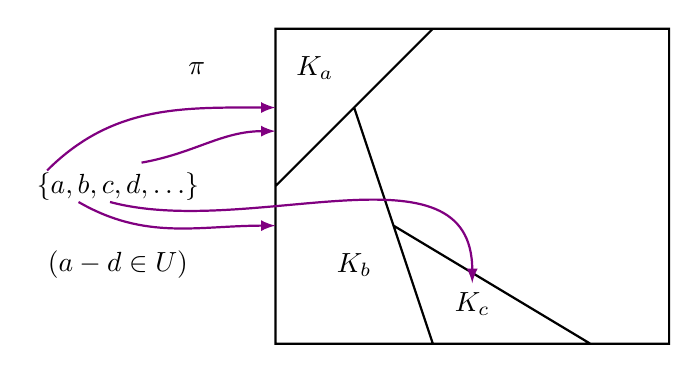
\begin{tikzpicture}
        \draw node at (3, 3.5) {$\pi$}
            node (set) at (2, 2) {$\{a,b,c,d,\ldots\}$}
            node [below of=set] {\normalsize$(a - d \in U)$}
            node (Ka) at (4.5, 3.5) {$K_a$}
            node (Kb) at (5, 1) {$K_b$}
            node (Kc) at (6.5, 0.5) {$K_c$}
            coordinate (a) at (1.1, 2.2)
            coordinate (b) at (1.5, 1.8)
            coordinate (c) at (1.9, 1.8)
            coordinate (d) at (2.3, 2.3);

        % \foreach \x in {1, 1.5, ..., 9}
        %     \foreach \y in {0, 0.5, ..., 4}
        %         \fill[black] (\x, \y) circle (1pt);

        % \foreach \pt in {a, b, c, d}
        %     \fill[red] (\pt) circle (1pt);

        \draw[thick] (4, 0) rectangle (9, 4)
            (4, 2) -- (6, 4)
            (5, 3) -- (6, 0)
            (5.5, 1.5) -- (8, 0);

        \draw[thick,violet,-latex] (a) to[out=45, in=180] (4, 3);
        \draw[thick,violet,-latex] (b) to[out=-30, in=180] (4, 1.5);
        \draw[thick,violet,-latex] (c) to[out=-15, in=90] (Kc);
        \draw[thick,violet,-latex] (d) to[out=10, in=180] (4, 2.7);
    \end{tikzpicture}

    \normalsize
    等价类:仿射子集(如何进一步描述其结构)

    商集:仿射子集构成的集合;商空间:商集上定义加法和数乘

    商映射:自然映射

    商空间的基与维数:两种方法
\end{figure}

\section{线性空间的积}

接下来的两节我们将综合应用之前所学习的基本知识,介绍两个重要的线性空间,即积空间和商空间,以及其上定义的线性映射. 在这两节中我们将完整地展示从定义的引入开始,如何研究一个线性空间,如何合理定义线性映射,如何应用前述知识综合地给出一些空间和映射的性质,这对于我们是一个重要的思维训练.

\subsection{线性空间的积的定义与性质研究}

我们首先探讨线性空间的积,或者积空间. 熟知集合有笛卡尔积运算,而线性空间是定义在集合上的代数结构,因此我们有一个自然的问题,即我们能否在多个线性空间的对应的集合的笛卡尔积上定义加法和数乘运算,使其成为一个线性空间?

答案是肯定的,但我们需要首先声明的一点是,构成笛卡尔积的这些线性空间必须定义在同一个数域上,否则新集合上的数乘我们将很难定义,因为数域不同我们将很难选择数乘的常数应该选择来自于哪个线性空间的数域.
\begin{definition}\label{def:8:积空间}
    设$V_1,V_2,\ldots,V_n$是数域$\mathbf{F}$上的线性空间,我们有如下三个定义:
    \begin{enumerate}
        \item 线性空间的积:
              \[V_1 \times V_2 \times \cdots \times V_n=\{(v_1,v_2,\ldots,v_n)\mid v_i \in V_i,\enspace i=1,2,\ldots,n\};\]

        \item 规定$V_1 \times V_2 \times \cdots \times V_n$上加法和数乘运算:
              \begin{enumerate}
                  \item 加法:$(v_1,v_2,\ldots,v_n)+(u_1,u_2,\ldots,u_n)=(v_1+u_1,v_2+u_2,\ldots,v_n+u_n)$;

                  \item 数乘:$\lambda(v_1,v_2,\ldots,v_n)=(\lambda v_1,\lambda v_2,\ldots,\lambda v_n)$.
              \end{enumerate}
    \end{enumerate}
\end{definition}

事实上我们很容易验证上述定义的线性空间的积在定义的加法和数乘运算下构成线性空间,我们将放在习题中供读者练习. 接下来我们要研究这一线性空间的性质. 事实上,我们早在有限维线性空间一节中就说明了,一个线性空间的核心结构就是其基和维数,因此我们首先研究它们. 事实上,对于积空间,它的基和维数的确定是非常符合我们的直觉的,我们来看一个例子:
\begin{example}
    求积空间$\mathbf{R}[x]_3\times\mathbf{R}^2$的一组基.
\end{example}

\begin{solution}
    我们知道$\mathbf{R}[x]_3$的一组基为$1,x,x^2$,而$\mathbf{R}^2$的一组基为$(1,0),(0,1)$. 很自然的想法是:我们可以先取$\mathbf{R}[x]_3$的一组基,$\mathbf{R}^2$的位置置零,然后反之取$\mathbf{R}^2$的一组基,$\mathbf{R}[x]_3$的位置置零,即$(1,(0,0)),\ (x,(0,0)),\ (x^2,(0,0)),\ (0,(1,0)),\ (0,(0,1))$. 我们很容易可以证明上述向量组满足基的两个条件:线性无关和张成空间.
\end{solution}

上述例子中的基的构造方法是很自然的,而且我们会发现,在这样取基的情况下积空间的维数很显然就是各个线性空间的维数之和. 我们可以很容易地推广到一般情况:
\begin{theorem}\label{thm:8:积空间维数}
    设$V_1,V_2,\ldots,V_n$是数域$\mathbf{F}$上的有限维线性空间,则$V_1 \times V_2 \times \cdots \times V_n$是有限维线性空间,且
    \[\dim(V_1 \times V_2 \times \cdots \times V_n)=\dim V_1+\dim V_2+\cdots+\dim V_n.\]
\end{theorem}

\begin{proof}
    我们取$V_i$的一组基,对这组基中每个向量,我们取$V_1 \times V_2 \times \cdots \times V_n$中的这样的向量:其中第$j$个位置为此向量,其余位置为零向量,这样我们遍历所有$V_i$和每个$V_i$的基向量我们就得到了$V_1 \times V_2 \times \cdots \times V_n$的一组基(线性无关和张成性是很容易验证的),这组基的长度(即维数)为$\dim V_1+\dim V_2+\cdots+\dim V_n$.
\end{proof}

\subsection{线性空间的积与直和}

本节我们将通过线性空间的积的角度来讨论直和的维数特点. 事实上,我们的手段就是构造线性映射,然后利用线性映射基本定理来得到结论.
\begin{theorem}\label{thm:8:积与直和}
    设$U_1,U_2,\ldots,U_n$是$V$的子空间,我们定义线性映射$\sigma:U_1 \times U_2 \times \cdots \times U_n \to U_1+U_2+\cdots+U_n$,使得$\sigma(u_1,u_2,\ldots,u_n)=u_1+u_2+\cdots+u_n$,则$U_1+U_2+\cdots+U_n$是$V$的直和$\iff \sigma$是双射.
\end{theorem}

\begin{proof}
    \begin{enumerate}
        \item 充分性:设$\sigma$是双射,则$\sigma$首先是单射. 根据单射的等价条件,我们有$\ker \sigma=\{0\}$,即$u_1+u_2+\cdots+u_n=0$必须有$u_1=u_2=\cdots=u_n=0$,而这正是\autoref{thm:4:直和等价命题} 中直和的等价条件;

        \item 必要性:设$U_1+U_2+\cdots+U_n$是直和,我们证明$\sigma$是单的、满的:
              \begin{enumerate}
                  \item 单射:设$\sigma(u_1,u_2,\ldots,u_n)=0$,即$u_1+u_2+\cdots+u_n=0$,由直和的等价条件可知$u_1=u_2=\cdots=u_n=0$,即$\sigma$的核空间只有出发空间零元,故是单射;

                  \item 满射:实际上是由这个线性映射的定义直接保证的. $\forall u \in U_1+U_2+\cdots+U_n$,根据和的定义一定有分解$u=u_1+u_2+\cdots+u_n$,其中$u_i \in U_i$,因此根据$\sigma$的定义$\sigma(u_1,u_2,\ldots,u_n)=u$,即任意$u$我们都可找到原像,故是满射.
              \end{enumerate}
    \end{enumerate}
\end{proof}

事实上在证明中我们看到,$\sigma$的定义保证了其满射性,因此定理中最后的双射改为单射也是统一的. 通过这一定理我们可以直接得出以下结论:
\begin{theorem}
    设$U_1,U_2,\ldots,U_n$是有限维线性空间$V$的子空间,则$U_1+U_2+\cdots+U_n$是$V$的直和$\iff \dim(U_1+U_2+\cdots+U_n)=\dim U_1+\dim U_2+\cdots+\dim U_n$.
\end{theorem}

\begin{proof}
    根据\autoref{thm:8:积与直和},$U_1+U_2+\cdots+U_n$是$V$的直和$\iff \sigma$是双射. 我们很容易验证$\sigma$是线性映射,而线性双射我们又称同构映射,同构映射的出发空间和到达空间维数相等,因此$\sigma$是双射$\iff \dim(U_1 \times U_2 \times \cdots \times U_n)=\dim(U_1+U_2+\cdots+U_n)$,最后根据\autoref{thm:8:积空间维数} 积空间的维数可知定理成立.
\end{proof}

这里我们用同构映射完成证明,如果对同构不熟悉的可以回顾定义和等价条件,或者自己用线性映射基本定理进行推导. 由此,我们通过在积空间上定义映射,结合\hyperref[thm:6:线性映射基本定理]{线性映射基本定理}(或同构)得到了\autoref{thm:4:直和等价命题} 中关于维数的命题. 总结而言,在积空间的讨论中我们展现了一个比较完整地学习路径:从定义积空间的想法(来源于集合的笛卡尔积),到如何自然地定义出这一空间的加法和数乘运算,然后研究构造出的空间的基本结构有什么特点,然后进一步构造其上线性映射,得到一些其他的结论. 这一路径的每一步都是非常自然的,而且是学习一个数学概念的常见思路,希望读者不仅是在线性代数中体会到这种学习路径,在其他数学课甚至其他学科中都能总结出这样一条引入—定义—性质—应用的自然路径.

最后我们再看一个拓展的问题,我们希望进一步看到构造同构映射带来的研究问题的方便性:
\begin{example}
    设$V_1,V_2,\ldots,V_n,W$是数域$\mathbf{F}$上的线性空间,证明:$\mathcal{L}(V_1 \times V_2 \times \cdots \times V_n,W)$与$\mathcal{L}(V_1,W) \times \mathcal{L}(V_2,W) \times \cdots \times \mathcal{L}(V_n,W)$同构.
\end{example}
有的读者可能看见这题就会觉得非常简单,因为有限维线性空间的前提下二者维数显然相同,然而我们这里并未限定有限维线性空间,因此需要读者自己构造同构映射.

\begin{solution}
    $\forall f\in \mathcal{L}(V_1 \times V_2 \times \cdots \times V_n,W)$,我们定义$f_i:V_i\to W(i=1,2,\ldots,m)$满足
    \[f_i(v_i)=f(0,\ldots,0,v_i,0,\ldots,0),\]
    其中$v_i$位于第$i$个位置,其余位置为零向量.

    定义$\varphi:\mathcal{L}(V_1 \times V_2 \times \cdots \times V_n,W)\to \mathcal{L}(V_1,W) \times \mathcal{L}(V_2,W) \times \cdots \times \mathcal{L}(V_n,W)$,使得$\varphi(f)=(f_1,f_2,\ldots,f_m)$,则接下来我们要验证$\varphi$就是我们要求的同构映射.
\end{solution}

\section{对偶空间与对偶映射}

本节我们将开始讨论矩阵的另一种很基本的运算:转置. 我们延续之前讨论的风格,首先介绍运算与线性映射之间的关联,然后再讨论其运算性质. 当然,转置与线性映射的关联不再像之前的那样简单明了,而是要首先引入线性空间和线性映射对偶的概念. 注意,这部分内容只在《线性代数应该这样学》中要求,只学习《大学数学:代数与几何》的读者可以选择性略过有关对偶的知识.

\subsection{对偶空间}

说起对偶,我们并不陌生,这一词语一路陪伴了我们从小学到高中的语文课,有``整齐匀称''之美. 在经济学中,我们可以将企业给定生产成本最大化产出的问题,和给定产出最小化成本的问题视为对偶. 我们自然的想法是,要定义线性空间的对偶,那么应当也是与原先的线性空间有着某种一一对应的关系. 接下来我们将开始定义线性空间的和对偶映射,然后逐步挖掘其中匀称之美.

我们首先回顾一下在\autoref{def:3:线性映射的定义} 中定义的线性泛函的概念:
\begin{definition}[线性泛函] \index{xianxingfanhan@线性泛函 (linear functional)}
    线性空间$V(\mathbf{F})$上的\term{线性泛函}是从$V$到$\mathbf{F}$的线性映射,即线性泛函是$\mathcal{L}(V,\mathbf{F})$中的元素.
\end{definition}
有时我们也将线性泛函称为线性函数,实际上它们都表示将$V$中向量映射到数域上的线性映射. 我们来看几个线性泛函的例子:
\begin{enumerate}
    \item 定义$\sigma:\mathbf{F}^n\to\mathbf{F}$为$\sigma(x_1,\ldots,x_n)=c_1x_1+\cdots+c_nx_n$,其中$c_1,\ldots,c_n\in\mathbf{F}$,则$\sigma$是线性泛函;

    \item 定义$\sigma:\mathbf{R}[x]_n\to\mathbf{R}$为$\sigma(p(x))=\displaystyle\int_0^1p(x)\mathrm{d}x$,则$\sigma$是线性泛函.
\end{enumerate}

我们知道,全体$V$到$\mathbf{F}$的线性映射构成的集合$\mathcal{L}(V,\mathbf{F})$也是一个线性空间(因为这只是$\mathcal{L}(V_1,V_2)$的特例),我们将其定义为线性空间$V$的对偶空间:
\begin{definition}[对偶空间] \index{duioukongjian@对偶空间 (dual space)}
    设$V$是数域$\mathbf{F}$上的线性空间,称$\mathcal{L}(V,\mathbf{F})$为$V$的\term{对偶空间},记作$V^*$.
\end{definition}

即线性空间$V$的对偶空间是其上所有线性泛函构成的线性空间. 事实上,我们知道对于有限维线性空间$V_1$和$V_2$而言,若$\dim V_1=n$,$\dim V_2=m$,则$\mathcal{L}(V_1,V_2)$的维数为$mn$. 因此对偶空间$V^*$的维数就是$\dim V$,因为数域构成的线性空间$\mathbf{F}(\mathbf{F})$维数显然为1,因为乘法单位元1就可以作为一组基(1自身线性无关,然后1数乘$\mathbf{F}$中的元素可以得到所有元素,当然同理只要是非零元就可以作为基).

有同学可能会想到$\mathbf{C}(\mathbf{R})$的维数为2,然而如果翻回线性映射的定义就会发现,我们要求两个线性空间的数域是一致的,所以$V(\mathbf{F})$上的线性泛函一定是到$\mathbf{F}(\mathbf{F})$上的.

沿着我们之前研究积空间和商空间的思路,接下来我们的目标非常明确:找到对偶空间的一组基. 我们可以考虑这样一个问题,假定$V$的维数为$n$,其一组基为$\alpha_1,\ldots,\alpha_n$. 由\autoref{thm:5:线性映射唯一确定} 可知,$V$上任一线性泛函$f$都可以由其在$\alpha_1,\ldots,\alpha_n$下的像$f(\alpha_1),\ldots,f(\alpha_n)$唯一确定. 我们考虑如下映射:
\begin{align*}
    \sigma:V^* & \to\mathbf{F}^n                         \\
    f          & \mapsto(f(\alpha_1),\ldots,f(\alpha_n))
\end{align*}
根据唯一确定性我们很容易证明可知$\sigma$是一个线性双射(即同构映射),事实上这也与$V^*$维数为$n$是相符的. 由于同构映射具有保持向量组线性相关性的特点,我们取$\mathbf{F}^n$的自然基$e_1,\ldots,e_n$,则$\sigma^{-1}(e_1),\ldots,\sigma^{-1}(e_n)$就是$V^*$的一组基,我们称其为\term{对偶基}\index{duiouji@对偶基 (dual basis)},记作$f_1,\ldots,f_n$.

我们进一步探究对偶基的性质,根据上面的定义我们知道$f_i=\sigma^{-1}(e_i)$,即$\sigma(f_i)=e_i$,根据$\sigma$定义即$f_i$在$\sigma$下的像$(f(\alpha_1),\ldots,f(\alpha_n))=e_1=(0,\ldots,0,1,0,\ldots,0)$,即第$i$个分量为1,其余分量为0,即$f_i(\alpha_j)=\delta_{ij}$,其中$\delta_{ij}$为Kronecker记号,展开写即
\[f_i(\alpha_j)=\begin{cases}
        1 & i=j     \\
        0 & i\neq j
    \end{cases}\]
这样我们便得到了对偶基. 我们上面的构造利用的是同构映射,因此无需证明线性无关和张成. 实际上直接证明也并不困难,我们将放在习题中供读者练习.

事实上,通过对偶基的表示我们很容易看出对偶基和原空间基的一一对应关系,即对偶基的某个向量(实际上是映射)只有在原空间对应位置的向量下的像才为1,其余向量下的像都为0. 讲到这里,可能很多读者已经觉得十分抽象了,我们可以理一下思路,对偶空间的定义就是全体线性泛函$V^*=\mathcal{L}(V,\mathbf{F})$,因此它的维数显然和$V$相等,并且我们通过了一个同构映射得到了对偶空间的基的表示. 因为对偶空间中的元素是线性映射,因此基向量也只不过是满足一定条件的线性映射罢了,只是这里的表达可能略微复杂不够直观,但我们可以通过例子来熟悉:
\begin{example}
    设$V=\mathbf{R}[x]_3$,对于$g(x)\in V$,定义:
    \[f_1(g(x))=\displaystyle\int_0^1g(x)\,\mathrm{d}x,\enspace f_2(g(x))=\int_0^2g(x)\,\mathrm{d}x,\enspace f_3(g(x))=\int_0^{-1}g(x)\,\mathrm{d}x,\]
    \begin{enumerate}
        \item 证明:$f_1,f_2,f_3$是$V^*$的一组基;

        \item 求出$V$的一组基$g_1(x),g_2(x),g_3(x)$,使得$f_1,f_2,f_3$是$g_1,g_2,g_3$的对偶基.
    \end{enumerate}
\end{example}

\begin{solution}

\end{solution}

\subsection{对偶映射}

接下来我们将介绍一个看起来可能更为抽象的概念——对偶映射. 如果我们有一个线性映射$\sigma:V\to W$,对偶映射的自然想法就是出发空间和到达空间变为对偶空间,于是我们有如下定义:
\begin{definition}[对偶映射] \index{duiouyingshe@对偶映射 (dual map)}
    设$\sigma:V\to W$是线性映射,定义$\sigma^*:W^*\to V^*$为$\sigma^*(f)=f\circ\sigma,\forall f\in W^*$,则称$\sigma^*$为$\sigma$的\term{对偶映射}.
\end{definition}
定义可能略显抽象,我们做一下说明:
\begin{enumerate}
    \item 看定义$\sigma^*(f)=f\circ\sigma,\enspace\forall f\in W^*$,实际上对偶映射只是把自变量$f$复合了一下原映射$\sigma$. 定义式很好记忆,接下来的各个证明都要熟练使用这一定义;

    \item 因为$\sigma^*(f)=f\circ\sigma,\enspace\forall f\in W^*$,其中$\sigma:V\to W,\enspace f:W\to\mathbf{F}$,由映射复合的定义可知$\sigma^*(f):V\to\mathbf{F}$,因此$\sigma^*$的出发空间是$W^*$(参数$f$所在空间),到达空间是$V^*$(像$\sigma^*(f)$所在空间),故$\sigma^*:W^*\to V^*$;

    \item $\sigma^*$满足线性性,因此是线性映射,证明只需使用线性映射复合运算的性质:
          \begin{gather*}
              \sigma^*(f_1+f_2)=(f_1+f_2)\circ\sigma=f_1\circ\sigma+f_2\circ\sigma=\sigma^*(f_1)+\sigma^*(f_2) \\
              \sigma^*(\lambda f)=(\lambda f)\circ\sigma=\lambda(f\circ\sigma)=\lambda\sigma^*(f)
          \end{gather*}

    \item 对偶映射还有以下运算性质:
          \begin{enumerate}
              \item $\forall\sigma,\tau\in\mathcal{L}(V,W),\enspace (\sigma+\tau)^*=\sigma^*+\tau^*$;

              \item $\forall\sigma\in\mathcal{L}(V,W),\enspace \forall\lambda\in\mathbf{F},\enspace (\lambda\sigma)^*=\lambda\sigma^*$;

              \item $\forall\sigma\in\mathcal{L}(V,W),\enspace \forall\tau\in\mathcal{L}(W,U),\enspace (\tau\sigma)^*=\sigma^*\tau^*$.
          \end{enumerate}
          注意这里的前两点也是线性性质,但前面是指线性映射,是映射对于自变量的线性性,这里可以将$^*$看成一种运算,这种运算作用于对偶映射,具有线性性. 我们简要证明一下这三条性质:

          \begin{proof}
              \begin{enumerate}
                  \item $(\sigma+\tau)^*(f)=(f\circ(\sigma+\tau))=(f\circ\sigma)+(f\circ\tau)=\sigma^*(f)+\tau^*(f)=(\sigma^*+\tau^*)(f)$;

                  \item $(\lambda\sigma)^*(f)=(f\circ(\lambda\sigma))=(\lambda(f\circ\sigma))=\lambda(f\circ\sigma)=\lambda\sigma^*(f)=(\lambda\sigma^*)(f)$;

                  \item $(\tau\sigma)^*(f)=(f\circ(\tau\sigma))=((f\circ\tau)\circ\sigma)=\sigma^*(f\circ\tau)=\sigma^*(\tau^*(f))=(\sigma^*\tau^*)(f)$.
              \end{enumerate}
          \end{proof}
          这里的$f$是任意的,因此这三条性质成立. 其中每一条最后一个等号我们回顾线性映射加法、数乘和复合的定义就会发现这一等号就是定义.
\end{enumerate}
这里希望读者能理解我们分点逐步加深理解的整理方式的良苦用心,事实上就是从简单的概念是什么开始,然后清晰地梳理出各种性质. 将来读者在其他课程中学习到了抽象的新概念,也可以试图做这样的整理,更符合一般的学习逻辑.

按照惯例,接下来我们要尝试使用线性映射基本定理研究对偶映射像空间和核空间的性质,然后得到一些推论. 我们从下面几个方面逐步深入讨论:
\begin{enumerate}
    \item 零化子:为了下面进一步的研究,我们首先要给出零化子的概念:
          \begin{definition}[零化子] \index{linghuazi@零化子 (annihilator)}
              对于线性空间$V$的子空间$U$,定义$U$的\term{零化子}$U^0$为
              \[U^0=\{\varphi\in V^*\mid\varphi(u)=0,\forall u\in U\}.\]
          \end{definition}

          对于零化子,我们有以下说明:
          \begin{enumerate}
              \item 根据定义,$U$的零化子实际上就是把$U$中向量全部映射为0的线性泛函;

              \item 我们很容易证明:$U^0$是$V^*$的子空间:
                    \begin{enumerate}
                        \item 非空:$0\in U^0$,零映射一定在$U^0$中;

                        \item 运算封闭:$\forall\varphi_1,\varphi_2\in U^0,\enspace \forall\lambda\in\mathbf{F}$,有
                              \begin{gather*}
                                  (\varphi_1+\varphi_2)(u)=\varphi_1(u)+\varphi_2(u)=0,\enspace\forall u\in U \\
                                  (\lambda\varphi_1)(u)=\lambda\varphi_1(u)=0,\enspace\forall u\in U
                              \end{gather*}
                              因此$\varphi_1+\varphi_2\in U^0,\enspace \lambda\varphi_1\in U^0$;
                    \end{enumerate}

              \item 既然零化子是子空间,那么我们对其基和维数就会十分感兴趣. 事实上,根据零化子$U^0$的定义是将子空间$U$完全映射为0,根据\autoref{thm:5:线性映射唯一确定},这等价于$U^0$中的元素将子空间$U$的基全部映为0. 设$U$的一组基为$\alpha_1,\ldots,\alpha_s$,则$U^0$中的元素$\varphi$满足
                    \begin{equation}\label{eq:9:零化子基}
                        \varphi(\alpha_1)=\cdots=\varphi(\alpha_s)=0.
                    \end{equation}
                    将这组基扩充成$V$的基$\alpha_1,\ldots,\alpha_s,\alpha_{s+1},\ldots,\alpha_n$,则$V^*$的对偶基为$f_1,\ldots,f_n$,其中$f_i(\alpha_j)=\delta_{ij}$,因此满足\autoref{eq:9:零化子基} 的$V^*$的基向量只有$f_{s+1},\ldots,f_n$. 我们自然猜想这就是$U^0$的一组基. 我们来验证:
                    \begin{enumerate}
                        \item 线性无关:证明是平凡的,因为$f_1,\ldots,f_n$是$V^*$的一组基,基向量组线性无关,因此其子向量组线性无关(可以回顾线性相关性的几种理解);

                        \item 张成空间:设$\varphi\in U^0$,由于首先有$\varphi\in V^*$,则它可以被$f_1,\ldots,f_n$线性表示,即
                              \begin{equation}\label{eq:9:零化子线性表示}
                                  \varphi=\lambda_1f_1+\cdots+\lambda_nf_n,\enspace \lambda_1,\ldots,\lambda_n\in\mathbf{F}.
                              \end{equation}
                              根据\autoref{thm:5:线性映射唯一确定} 可知,$\varphi$被其在$\alpha_1,\ldots,\alpha_n$下的像唯一确定. 由于$\varphi\in U^0$,因此$\varphi(\alpha_1)=\cdots=\varphi(\alpha_s)=0$,代入\autoref{eq:9:零化子线性表示} 可得$\lambda_1=\cdots=\lambda_s=0$.

                              进一步我们将$\alpha_{i},\enspace i=s+1,\ldots,n$代入\autoref{eq:9:零化子线性表示} 可得$\lambda_{i}=\varphi(\alpha_i)$,因此$\varphi$可以被$f_{s+1},\ldots,f_n$线性表示为
                              \[\varphi=\varphi(\alpha_{s+1})f_{s+1}+\cdots+\varphi(\alpha_n)f_n.\]
                    \end{enumerate}
                    因此我们可以根据证明过程得到$U^0$的一组基为$f_{s+1},\ldots,f_n$,维数为$n-s$,更一般地我们有
                    \[\dim U^0=\dim V-\dim U.\]
          \end{enumerate}

    \item 对偶映射核空间与像空间的性质:我们不加证明地给出四个结论,它们对应《线性代数应该这样学》的3.107和3.109. 笔者认为教材给出的证明非常清楚,因此不再赘述.
          \begin{theorem}\label{thm:9:对偶映射像和核的性质}
              设$V$和$W$都是有限维线性空间,$\sigma\in\mathcal{L}(V,W)$,则
              \begin{enumerate}
                  \item $\ker\sigma^*=(\im\sigma)^0$;

                  \item $\dim\ker\sigma^*=\dim\ker\sigma+\dim W-\dim V$;

                  \item $\dim\im\sigma^*=\dim\im\sigma$;

                  \item $\im\sigma^*=(\ker\sigma)^0$.
              \end{enumerate}
          \end{theorem}

          事实上很多情况下我们也并不需要背诵这些性质,一方面这只是几个由前面更为基本的概念和定理导出的性质,不具一般性,并且是为了下面更重要的结论铺垫;另一方面即使一定要记忆,它们很强的对称性使得记忆难度不大.

          这一定理有一个非常关键的推论,其重要性大于上述定理,证明非常简单,见《线性代数应该这样学》3.108和3.110:
          \begin{corollary}\label{cor:9:对偶映射单满射}
              设$V$和$W$都是有限维线性空间,$\sigma\in\mathcal{L}(V,W)$,则
              \begin{enumerate}
                  \item $\sigma$是单射当且仅当$\sigma^*$是满射;

                  \item $\sigma$是满射当且仅当$\sigma^*$是单射.
              \end{enumerate}
          \end{corollary}
\end{enumerate}

\subsection{双重对偶空间}

实际上,对偶空间有一个弊端,我们发现$V^*$的对偶基的选取是与$V$的基的选取有关的,因为我们需要首先确定$V$的一组基$\alpha_1,\ldots,\alpha_n$,然后才能得到$V^*$的对偶基$f_1,\ldots,f_n$,满足$f_i(\alpha_j)=\delta_{ij}$,其中$\delta_{ij}$为Kronecker记号.

事实上这并不美观,因为如果我们尝试定义$V$和$V^*$之间的同构,由于这两个空间两组基的强相关性,我们一般需要有如下定义:
\begin{align*}
    \sigma:V                       & \to V^*                   \\
    \alpha=\sum_{i=1}^nx_i\alpha_i & \mapsto\sum_{i=1}^nx_if_i
\end{align*}
我们会发现,这一映射的定义中$\alpha_i$和$f_i$都离不开选取$V$的一组基$\alpha_1,\ldots,\alpha_n$,更通俗地说,在我们取定了$V$的一组基前,我们甚至写不出$V$和$V^*$之间的同构!

为了更容易地理解这一点,我们可以回想以往的线性映射的定义,例如最简单的
\[\sigma(x_1,x_2,x_3)=(x_1-x_2,x_1+x_3,x_2-x_3),\]
我们要求一个任意元素的像,例如$\sigma(1,2,3)$,我并不需要取$\mathbf{R}^3$的自然基还是其他的基也能知道像为$(-1,4,-1)$,然而$V$和$V^*$之间的同构$\sigma$作用于任意向量$\alpha$后的像$\sigma(\alpha)$在未确定$V$的基前是未定义的!我们一定需要$V$的基才能有坐标$x_i$,然后再利用这个坐标结合像空间的基(这组基和$V$的基是有关的)才能得到像,因此这里的同构映射是非常不美观的.

有的读者可能会质疑,即$V$和$V^*$之间的同构真的一定需要建立在取定$V$的基的基础上吗?事实上的确是需要的,更规范的表述需要进一步学习范畴学等更为深入的数学知识,这里我们只给出直觉:因为同构映射实际上建立的是两个空间基的一一对应关系,然而$V^*$的基本身就依赖于$V$的基的选取,因此我们很难在定义同构映射时避免需要先确定$V$的基这一前提.

因此我们会尝试研究$V$的对偶空间$V^*$的对偶空间$V^{**}$,我们称之为\term{双重对偶空间}\index{duioukongjian!shuangchong@双重 (double dual space)}. 由于$V^*=\mathcal{L}(V,\mathbf{F})$,因此$V^{**}=\mathcal{L}(V^*,\mathbf{F})=\mathcal{L}(\mathcal{L}(V,\mathbf{F}),\mathbf{F})$,因此$V^**$中的元素是这样的线性映射:它的自变量是$V$上的线性泛函,它将这一线性泛函映到一个数.

我们知道$\dim V=\dim V^*$,故$V^*$也和其对偶空间有相同的维数,即$\dim V^*=\dim V^{**}$,故$\dim V=\dim V^{**}$,因此我们可以尝试构造一个同构映射$\sigma:V\to V^{**}$,使得这一映射不依赖于$V$的基的选取. 我们发现这样的映射是存在的,我们来跟着下面这个例子逐步说明:
\begin{example}
    设$V$为有限维线性空间. 我们定义$\tau:V\to V^{**}$为
    \[(\tau(\alpha))(f)=f(\alpha),\enspace\forall \alpha\in V,\enspace f\in V^*.\]
    \begin{enumerate}
        \item 证明:$\tau$是线性映射;

        \item 证明:若$\sigma\in\mathcal{L}(V,V)$,则$\sigma^{**}\circ\tau=\tau\circ\sigma$,这里$\sigma^{**}$是$\sigma^*$的对偶映射;

        \item 证明:$\tau$是$V$到$V^{**}$的同构映射.
    \end{enumerate}
\end{example}

\begin{solution}

\end{solution}

我们发现这一同构映射不需要先确定$V$的基就可以定义,因此相对于$V$与$V^*$间的同构映射更为自然. 在范畴学中,我们称这样的映射为
\term{自然同构}\index{tonggou!ziran@自然同构 (natural isomorphism)},它不依赖于选取的基,一直客观存在着,就好像在等着我们发现一样,而$V$与$V^*$间的同构映射则需要通过我们先取出$V$的基才能定义,因此缺少了这样``自然''的客观存在的感觉.

事实上本节的讨论是比较抽象的,我们只能通过一些例子和描述来直观理解其中核心的思想,即自然同构中``自然''的含义(不依赖于基的选取). 我们长篇的论述的核心就是直观地告诉读者,$V$和$V^*$之间找不到自然同构,但$V$和$V^{**}$之间存在. 更深入、严谨的讨论可能需要读者进一步学习范畴学的相关知识才能全面理解.

\section{对偶映射的矩阵}

有了前述内容的铺垫,本节我们将最终给出对偶映射的矩阵. 我们首先介绍矩阵转置的概念,然后说明对偶为什么与转置相关.
\begin{definition}[转置] \index{zhuanzhi@转置 (transpose)}
    设$A=\begin{pmatrix}
            a_{11} & a_{12} & \cdots & a_{1n} \\
            a_{21} & a_{22} & \cdots & a_{2n} \\
            \vdots & \vdots & \ddots & \vdots \\
            a_{m1} & a_{m2} & \cdots & a_{mn}
        \end{pmatrix}$,称$\begin{pmatrix}
            a_{11} & a_{21} & \cdots & a_{m1} \\
            a_{12} & a_{22} & \cdots & a_{m2} \\
            \vdots & \vdots & \ddots & \vdots \\
            a_{1n} & a_{2n} & \cdots & a_{mn}
        \end{pmatrix}$为矩阵$A$的\term{转置},记作$A^\mathrm{T}$.
\end{definition}

简单来说,矩阵的转置就是矩阵的第$i$行变成了第$i$列(或者第$i$列变成了第$i$行,即行列互换),原先矩阵第$i$行第$j$列的元素转置后变为第$j$行第$i$列的元素,或者抽象表达为:
\[A=(a_{ij})_{m \times n},\enspace A^\mathrm{T}=(a'_{ji})_{n \times m},\enspace a_{ij}=a'_{ji}\]

接下来我们将说明对偶映射在对偶基下的矩阵就是原映射在原空间基下矩阵的转置:
\begin{theorem}
    $V$和$W$为有限维线性空间. $V$的一组基为$\alpha_1,\ldots,\alpha_n$,$W$的一组基为$\beta_1,\ldots,\beta_m$,它们对偶空间的基分别为$f_1,\ldots,f_n$和$g_1,\ldots,g_m$. 设$\sigma\in\mathcal{L}(V,W)$,它在上述$V$和$W$的基下的矩阵为$A=(a_{ij})_{m \times n}$,则$\sigma^*\in\mathcal{L}(W^*,V^*)$在上述对偶基下的矩阵为$C=(c_{ij})_{n \times m}=A^\mathrm{T}$.
\end{theorem}

\begin{proof}
    根据线性映射矩阵表示的定义,我们有
    \[\sigma^*(g_j)=\sum_{i=1}^nc_{ij}f_i,\enspace j=1,2,\ldots,m.\]
    上式左端根据对偶映射定义等于$(g_j\circ\sigma)$. 于是我们将等式两端均作用于$\alpha_k$上有
    \[(g_j\circ\sigma)(\alpha_k)=\sum_{i=1}^nc_{ij}f_i(\alpha_k)=\sum_{i=1}^nc_{ij}\delta_{ik}=c_{kj}.\]
    另一方面,根据映射复合的结合律以及线性映射矩阵表示的定义,我们有
    \[(g_j\circ\sigma)(\alpha_k)=g_j(\sigma(\alpha_k))=g_j\left(\sum_{i=1}^na_{ik}\beta_i\right)=\sum_{i=1}^na_{ik}g_j(\beta_i)=\sum_{i=1}^na_{ik}\delta_{ij}=a_{jk}.\]
    因此我们有$c_{kj}=a_{jk}$,即$C=A^\mathrm{T}$.
\end{proof}

可能由许多同学心存疑惑——我们为什么要费这么大劲介绍一个这么特别且抽象的概念然后引入转置?事实上对偶这一概念在数学中是非常重要的,在之后我们还将提起它,现在可以先留下一个美好的期待,相信在之后的学习中你会逐渐发现这一定义是自然而美妙的,而且其中蕴含的思想是有很大的应用价值的.

除此之外,在这一讲中笔者也反复强调,面对这一抽象的内容我们不要畏惧,我们可以先从是什么开始,熟练概念,然后理解相关的性质,例如我们在定义对偶映射的时候就强调先记住很好记忆的定义式,然后我们再说明它的出发空间、到达空间是什么,具有什么样的性质,不能一开始就妄图直接装下所有的概念、性质,这样只能使思维混乱且不知道自己学了什么. 我们应当学会将抽象的概念通过拆解成大家从小就习惯的``是什么''的教育和研究中更感兴趣的内容两部分进行梳理,从而更快地理解.

\vspace{2ex}
\centerline{\heiti \Large 内容总结}

事实上,这一讲是本讲义第一次接触技巧性较强的内容,我们的重点从之前对于定理的证明以及用例子巩固定理的应用转变为了对于一些技巧性的处理. 我们首先介绍了三类初等变换(请务必注意正文中强调的几个定义的细节),证明了任意可逆矩阵都可以被表示成若干初等矩阵的乘积,也基于此引出了第二种求解逆矩阵的方法——初等变换法,这也是我们未来最常用的方法. 除此之外,我们也联系了线性映射矩阵表示和初等变换,研究了高斯消元法背后的合理性.

接下来我们介绍了分块矩阵的基本运算性质,比较了分块矩阵和一般矩阵运算的异同(特别是乘法和转置),介绍了两种分块矩阵求逆的方法:其一直接设出逆矩阵,其二利用所谓打洞法(分块矩阵初等变换),其中打洞法是一个很重要的技巧,虽然教材列为小字部分,考试中一般不考察,但拥有这一技巧对我们未来证明很多结论都有很大的帮助. 最后我们介绍了矩阵方程的求解方法,本质而言介绍了几种基于初等变换的求解方法,读者理解其内涵即可.

\vspace{2ex}
\centerline{\heiti \Large 习题}

\vspace{2ex}
{\kaishu 龙生龙,凤生凤,华罗庚的学生会打洞.}
\begin{flushright}
    \kaishu
    ——线性代数教学俗语
\end{flushright}

\centerline{\heiti A组}
\begin{enumerate}
    \item 设$A$为三阶矩阵,将$A$的第二列加到第一列得到矩阵$B$,再对调$B$的2、3行得到单位矩阵. 令$P_1=\begin{pmatrix}1 & 0 & 0 \\ 1 & 1 & 0 \\ 0 & 0 & 1\end{pmatrix}\enspace
              P_2=\begin{pmatrix}1 & 0 & 0 \\ 0 & 0 & 1 \\ 0 & 1 & 0\end{pmatrix}$,试用$P_1$和$P_2$表示$A$.

    \item 设$A$为可逆矩阵,将$A$的第$i$行和第$j$行对调得到矩阵$B$,证明矩阵$B$可逆并求$AB^{-1}$.

    \item 设$A$为三阶可逆矩阵,且$P^{-1}AP=\begin{pmatrix}1 & 0 & 0 \\ 0 & 1 & 0 \\ 0 & 0 & 2\end{pmatrix}$,其中$P=(\alpha_1,\alpha_2,\alpha_3)$,令$Q=(\alpha_1+\alpha_2,\alpha_2,\alpha_3)$,求$Q^{-1}AQ$.

    \item 求下列矩阵的可逆的条件与逆矩阵:$\begin{pmatrix}
                  A & B \\ O & D
              \end{pmatrix},\enspace \begin{pmatrix}
                  O & B \\ C & D
              \end{pmatrix}$.
\end{enumerate}

\centerline{\heiti B组}
\begin{enumerate}
    \item 已知$\mathbf{R}^3$的基$B_1=\{\alpha_1,\alpha_2,\alpha_3\}$变为基$B_2=\{\xi_1,\xi_2,\xi_3\}$的变换矩阵为$A=(a_{ij})_{3 \times 3}$,求:
          \begin{enumerate}
              \item 基$B_3=\{\alpha_2,\alpha_1,\alpha_3\}$变为基$B_2$的变换矩阵;

              \item 基$B_4=\{-\alpha_1,\alpha_2,\alpha_3\}$变为基$B_2$的变换矩阵;

              \item 基$B_4$变为基$B_5=\{\xi_3,\xi_2,-\xi_1\}$的变换矩阵;

              \item 基$B_4$变为基$B_6=\{\xi_1+\xi_2,\xi_2+\xi_3,\xi_3+\xi_1\}$的变换矩阵.
          \end{enumerate}

    \item 设$P=\begin{pmatrix}
                  1 & 1 & 0 \\ 0 & 1 & 0 \\ 0 & 0 & 0
              \end{pmatrix}$,$Q=\begin{pmatrix}
                  0 & 0 \\ 1 & 0
              \end{pmatrix}$,定义$\mathbf{R}^{3\times 2}$上映射$\sigma(A)=PAQ$.
          \begin{enumerate}
              \item 验证$\sigma$是线性映射;

              \item 求$\ker\sigma$和$\im \sigma$;

              \item 求$\mathbf{R}^{3\times 2}$的两组基,使得$\sigma$关于这两组基的表示矩阵是对角矩阵.
          \end{enumerate}

    \item % 新题,需要答案
\end{enumerate}

\centerline{\heiti C组}
\begin{enumerate}
    \item 若$n$阶矩阵$A$的各阶左上角子块矩阵都可逆,则存在$n$阶下三角矩阵$B$,使得$BA$为上三角矩阵.

    \item 设$A$是数域$\mathbf{F}$上的$n$阶可逆矩阵,把$A$和$A^{-1}$做如下分块:
          \[A=\begin{pmatrix}
                  A_{11} & A_{12} \\ A_{21} & A_{22}
              \end{pmatrix},\enspace A^{-1}=\begin{pmatrix}
                  B_{11} & B_{12} \\ B_{21} & B_{22}
              \end{pmatrix}\]
          其中$A_{11}$是$l \times k$矩阵,$B_{11}$是$k \times l$矩阵,$l$,$k$是小于$n$的正整数. 用$W$表示$A_{12}X=0$的解空间,$U$表示$B_{12}Y=0$的解空间,其中$X$和$Y$为列向量,证明$W$与$U$同构.

    \item $A$的Schur补以及商等式$A/B=(A/C)/(B/C)$% 新题,需要答案
\end{enumerate}
